\chapter{Experiments and Results}
\label{S:Experiments}
%
To reliably measure the accuracy of a matching method on real images, we 
either need a set of image pairs tied by a homography, or we have to 
manually count the number of inliers. The latter becomes prohibitive for 
large numbers of (non-trivial) images. 

Mikolajczyk and Schmid  \cite{mikolajczyk2005performance} introduced a 
set of test images to compare the performance of feature detectors. The 
set covers different types of image variations, such as lighting change, 
blur, rotation, and viewpoint change. Inspired by this dataset (in 
particular the `Graf' image set) and motivated by the need for more 
image pairs featuring viewpoint changes, we have compiled a set of 8 
image pairs consisting of subjects taken from two different angles. The 
images are collected from Flickr's database of images published under a 
creative commons licence and feature murals, which makes it possible to 
relate points in the image pairs with a homography since most of the 
points in the images will be lying on a plane.  The images have been 
cropped to show the same motive and resized to $900\times 600$ pixels.  
This dataset will be referred to as the \emph{Murals} dataset.  
Figure~\ref{fig:murals} shows one image from each pair.

\begin{figure}[htb]
    \makebox[1.0\textwidth][c]{%
        \begin{subfigure}[t]{0.102\textwidth}
			\centering
			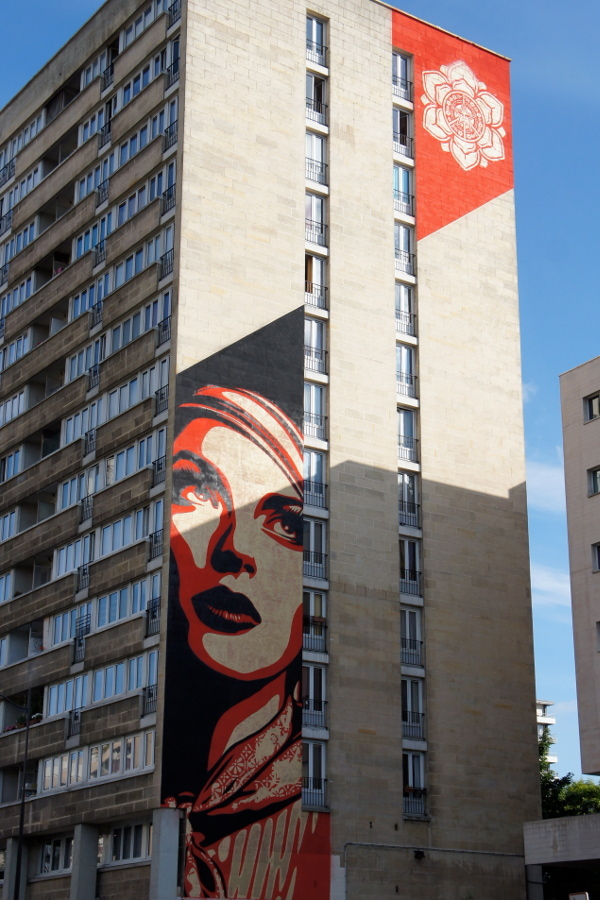
\includegraphics[width=\textwidth]{images/pair_example1}
			\label{fig:fairey1}
	\end{subfigure}%
		\enspace %add desired spacing between images, e. g. ~, \quad, 
		%(or a blank line to force the subfigure onto a new line)
        \begin{subfigure}[t]{0.102\textwidth}
			\centering
			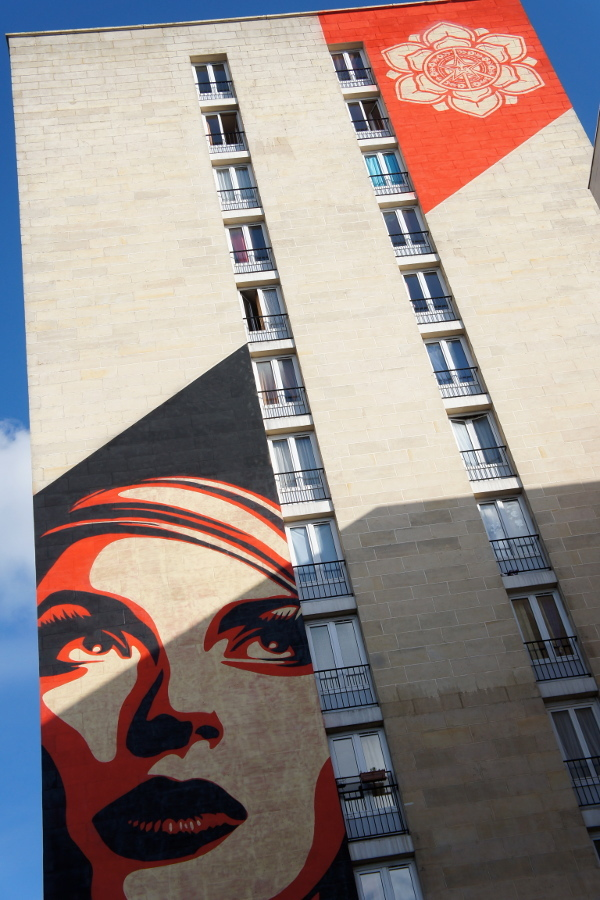
\includegraphics[width=\textwidth]{images/pair_example2}
			\label{fig:fairey2}
		\end{subfigure}%
		\enspace %
        \begin{subfigure}[t]{0.77\textwidth}
   		\centering
   		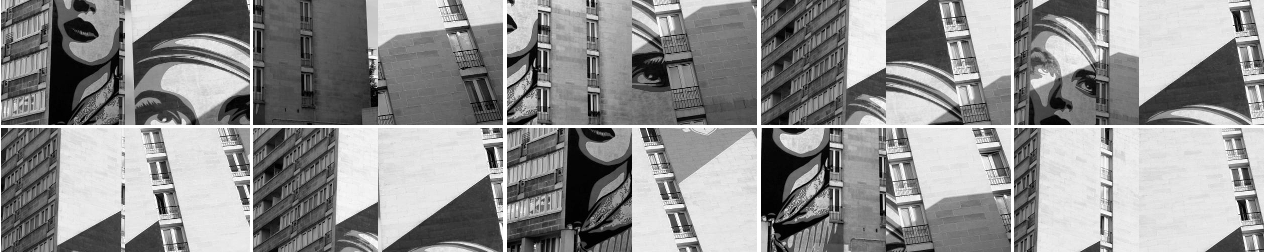
\includegraphics[width=\columnwidth]{images/crop_examples}
		\end{subfigure}%
	}%
	\caption{Sample test patches produced from an image pair.}
	\label{fig:fairey}
\end{figure}

\begin{figure*}[t]
	\centering
	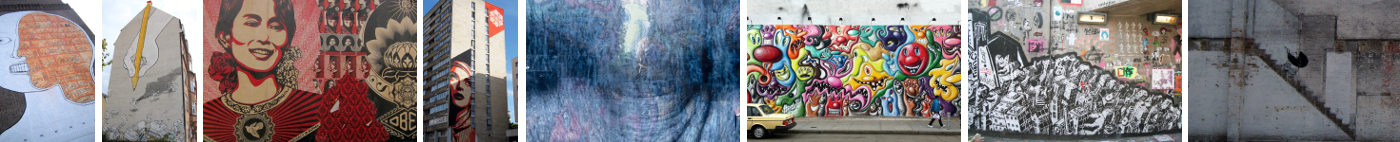
\includegraphics[width=\textwidth]{images/murals}
	\caption{Images in the \emph{Murals} test set.}
	\label{fig:murals}
\end{figure*}

\begin{figure}[htb]
	\centering
	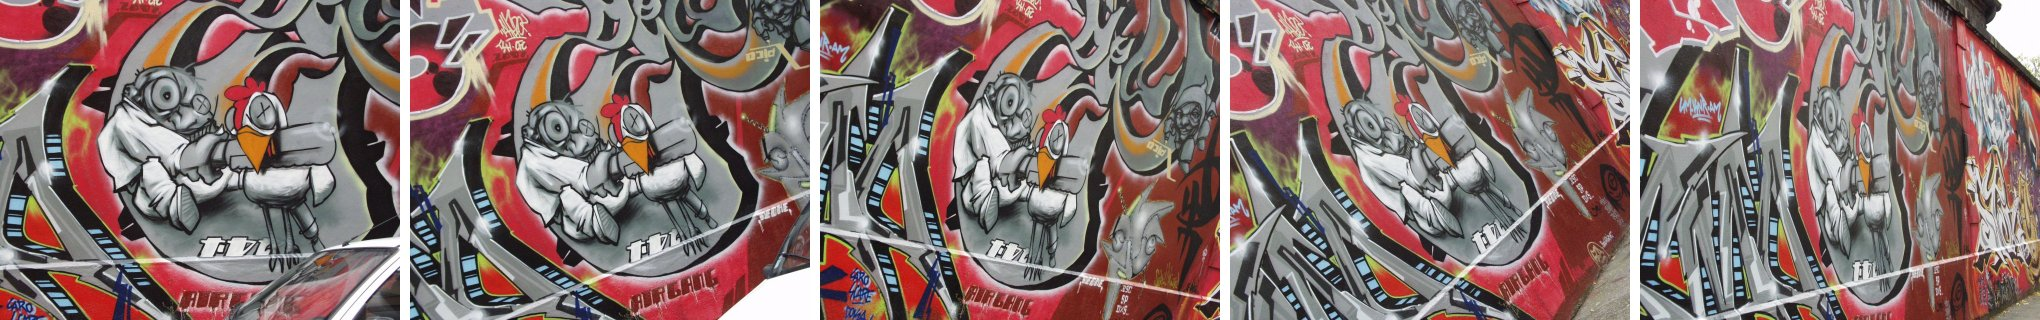
\includegraphics[width=\columnwidth]{images/graf12345.jpg}
	\caption{Images 1-5 of the Graf set from \cite{mikolajczyk2005performance}.}
	\label{fig:Graf}
\end{figure}


The comparison was done using the \emph{Murals} dataset 
(Figure~\ref{fig:murals}), the \emph{Graf} set (Figure~\ref{fig:Graf}) 
from \cite{mikolajczyk2005performance}, and two 
images\footnote{100\_1942.jpg and 100\_1941.jpg} from the Gallagher 
dataset \cite{gallagher2008} (Figure~\ref{fig:comparemirror}).

Test sets were generated from the image pairs by cropping square patches of
$250\!\times\!250$ pixels with a random vertical and horizontal offset.  
Given a source image pair, we produce 100 pairs of patches, which might or might not overlap.  
This ensures that patch pairs with no overlap still retain a general similarity to each 
other, while patches that do overlap often only share a small 
part of their area. Figure~\ref{fig:fairey} shows an example of 
possible pairs of test image patches produced from a source image pair.  
Producing $n$ such pairs allows us to test not just how well the 
matching algorithm performs on a variety of overlaps but also how many 
false positives we get on similar images that do not overlap at all. In 
practice the amount of overlap between pairs in a test set will depend 
on the overlap and viewpoint change in the source image pair.  To give a 
rough idea, Table~\ref{table:overlap} shows the overlap of patch pairs 
created from images 1 and 3 of the \emph{Graf} image set from 
\cite{mikolajczyk2005performance}.

\begin{table}[htb]
\caption{Overlap in the set of 100 patch pairs created from two images 
of the \emph{Graf} image set (Figure~\ref{fig:Graf}).}
\label{table:overlap}
    \centering
%   \small
\begin{tabular}{r*{3}{r}}
\hline
    Amount of overlap: & 0\% & $< 50$\% & $> 50$\%  \\
    \noalign{\smallskip}
	%
    Number of patch pairs: & 21 & 54 & 25 \\
    \hline
\end{tabular}
\end{table}

The results are presented as \emph{precision} versus \emph{recall} 
similar to \cite{ke2004pca} and \cite{mikolajczyk2005performance}.  
Recall corresponds to the number of correct matches over the total 
amount of possible correct matches in between the two images:
\begin{equation*}
	recall = \frac{\# ~ Correct ~ Matches}{\# ~ Total ~ Possible ~ 
	Matches}
\end{equation*}
This measure tells us how many thorough we are in finding all possible 
matches that could be made between the two images. To decide whether a 
match is correct, we use the following method:
Given a potential match between two pixels $p_1$ and $p_2$, $m = 
\left(p_1, p_2\right)$, and a homography $H$ relating the two images 
$I_1$ and $I_2$, we can calculate if $m$ is an inlier by checking if the 
two points satisfy the following criteria:
\begin{equation*}
\left\vert H p_1 - p_2 \right\vert + \left\vert H^{-1}p_2 - p_1 \right\vert < d_{\max}
\end{equation*}
That is, the distance between $p_1$ translated to $I_2$ and $p_2$ 
\emph{plus} the distance between $p_2$ translated to $I_1$ should be 
less than a certain threshold (we use $d_{\max}=5$ pixels here). To 
count the number of possible matches we go over all possible 
combinations of feature points between the two images, measure their 
distance and count how many lie within the threshold.
Precision on the other hand is measured by the amount of correct matches
over the total amount of matches returned:
\begin{equation*}
	precision = \frac{\# ~ Correct ~ Matches}{\# ~ Correct ~ Matches ~ + 
	~ \# ~ False ~ Matches}
\end{equation*}
This measures how accurate the set of returned matches from the 
algorithm is. An algorithm that returns only a few matches out of many, 
but most of them are correct will have a high precision and a low 
recall, where as an algorithm that returns almost all possible matches, 
both true and false will have a low precision but a high recall. The 
ideal matching algorithm will be both precise but also return as many 
correct matches as possible. However for many applications we only need 
enough correct matches to align to the images, in which case we care 
more about precision than recall. 


\section{Results}
\label{S:Results}

Figure~\ref{fig:result_graf} shows the results for 100 patch pairs 
generated from images 1 and 3 of the \emph{Graf} image set 
(cf.~Figure~\ref{fig:Graf}). The plot compares the accuracy of 
\emph{Ratio}, \emph{MM}, \emph{MMC}, \emph{Isomatch} and \emph{Spectral} 
as a function of the number of matches produced (which is achieved by 
varying thresholds over a certain range). The results show that 
\emph{MM} and \emph{MMC} consistently outperform \emph{Ratio}; 
\emph{MMC} generally lies 2-3 percentage points above \emph{MM} when 
both are performing at optimal accuracy.  The geometric matching methods 
\emph{Isomatch} and \emph{Spectral} outperform \emph{Ratio} but fall 
short of \emph{MM} and \emph{MMC}.


\begin{figure}[htb]
	\begin{subfigure}[c]{0.2\textwidth}
		\centering
		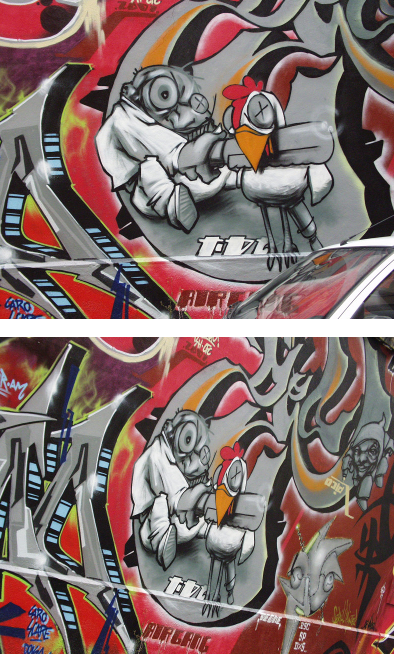
\includegraphics[width=\textwidth]{images/graf}
	\end{subfigure}%
	~ %add desired spacing between images, e. g. ~, \quad, \qquad		  
	%(or a blank line to force the subfigure onto a new line)
	\begin{subfigure}[c]{0.8\textwidth}
	\centering
	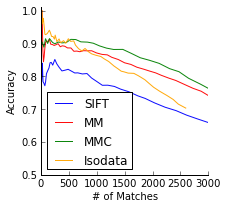
\includegraphics[width=\columnwidth]{images/result_graf}
	%\caption{Performance on Scharf}
	\end{subfigure}%
	\caption{Accuracy for image pair 1\&3 from the \emph{Graf} set. The 
	plot shows the result of 100 patch pairs generated from the source 
	images shown to the left. The x-axis shows the recall based on the 
accumulated amount of potential matches for all 100 patch pairs. }
	\label{fig:result_graf}
\end{figure}

To validate whether these results generalize to other images, we tested 
the four algorithms on the \emph{Murals} dataset as well as the 
\emph{Graf} pair tested above.  In total 900 different patch pairs were 
generated from 9 source image pairs.  The results are shown in Figure 
\ref{fig:result_accumulated}. 

\begin{figure}[htb]
	\centering
	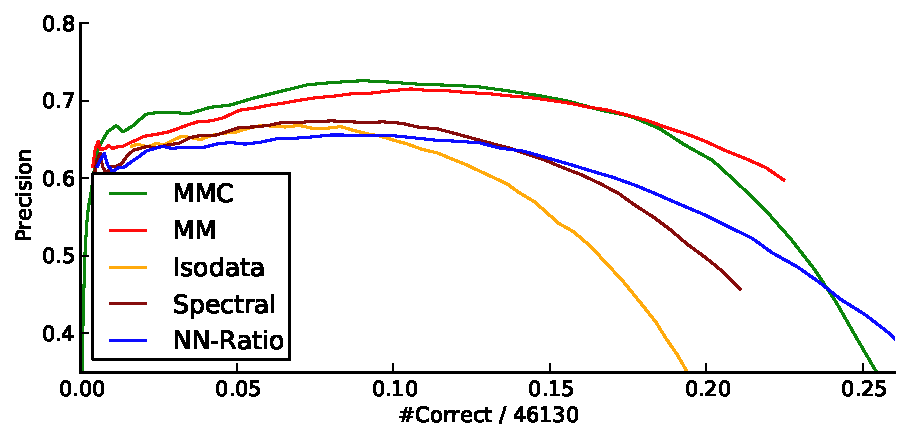
\includegraphics[width=\columnwidth]{images/result_accumulated}
	\caption{Results for 900 patch pairs extracted from the 
	\emph{Murals} dataset and the image pair 1\&3 from the \emph{Graf} 
	set.  The x-axis shows the recall based on the accumulated amount of 
potential matches for all patch pairs.}
	\label{fig:result_accumulated}
\end{figure}

To further investigate the impact of viewpoint changes, we tested the 
algorithms on the \emph{Graf} image set (Figure~\ref{fig:Graf}), which 
contains 5 images of the same mural taken with gradually increasing 
viewpoint changes.  The first images are almost identical, while the 
last are taken from very different angles. The results from   \emph{MMC} 
and \emph{Ratio} as shown in Figure~\ref{fig:result_viewpoint}, 
confirming that \emph{MMC} is generally superior to \emph{Ratio} across 
viewpoint changes.
The performance of \emph{MM} (not shown in the plot) is similar to 
\emph{MMC}.

\begin{figure}[htb]
	\centering
	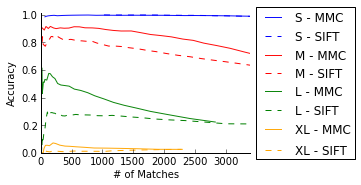
\includegraphics[width=1\textwidth]{images/result_viewpoint}
	\caption{Results for viewpoint changes using the \emph{Graf} set 
	from \cite{mikolajczyk2005performance}.  S: img1\&2; M: img1\&3; L: 
	img1\&4; XL: img1\&5.}
	\label{fig:result_viewpoint}
\end{figure}

In order to investigate whether a geometric algorithm can be improved by
pruning the initial matching set, we tested a hybrid algorithm 
\emph{Spectral-MMC} where matches are pruned by \emph{MMC} before being 
applied to \emph{Spectral}. The results are shown in 
Figure~\ref{fig:result_spectral-mmc} and show that \emph{Spectral-MMC} 
not only outperforms \emph{Spectral} but also improves on \emph{MMC} at 
similar recall rates, illustrating how a geometric algorithm can be 
complemented by a reliable non-geometric pruning of matches.

\begin{figure}[htb]
	\centering
	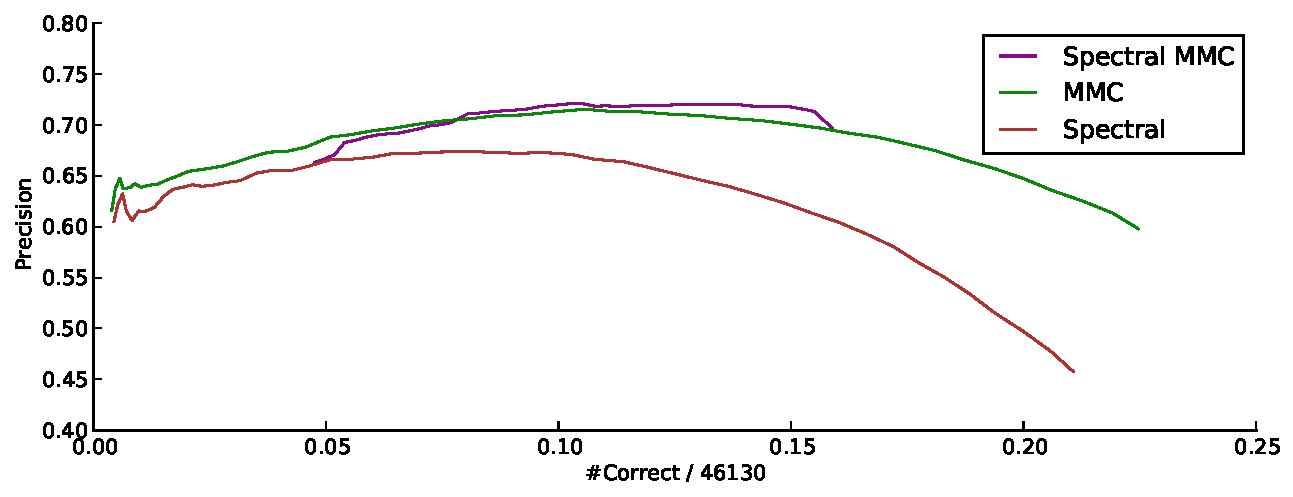
\includegraphics[width=1\textwidth]{images/result_spectral-mmc}
	\caption{Results for filtering matches with \emph{MMC} before 
	applying the \emph{Spectral} algorithm. The algorithm is tested on 
900 patch pairs extracted from the \emph{Murals} dataset and the image 
pair 1\&3 from the \emph{Graf} set. The x-axis shows the recall based on 
the accumulated amount of potential matches for all patch pairs.}
	\label{fig:result_spectral-mmc}
\end{figure}

Finally, as an example of a real life use case, 
Figure~\ref{fig:result_pitts} shows the results on 100 patch pairs 
generated from a typical holiday photo shot 
(Figure~\ref{fig:pitts_source}) featuring occlusion and a slight 
viewpoint change from the Gallagher dataset \cite{gallagher2008}.  The 
performance is comparable to the murals, despite the lack of a simple 
homographic mapping between the images.


\begin{figure}[htb]
	\begin{subfigure}[c]{.2\textwidth}
		\centering
		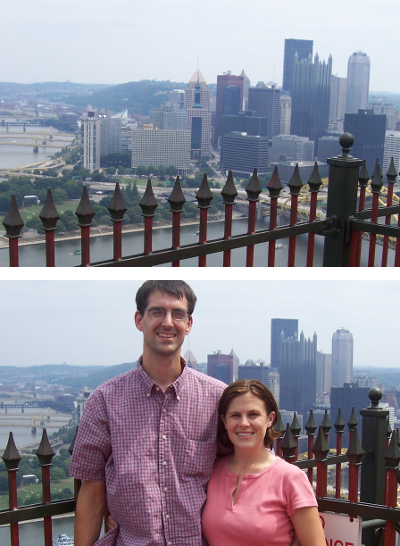
\includegraphics[width=\textwidth]{images/pitts}
	\end{subfigure}%
	~%add desired spacing between images, e. g. ~, \quad, \qquad
	%(or a blank line to force the subfigure onto a new line)
	\begin{subfigure}[c]{.8\textwidth}
	\centering
	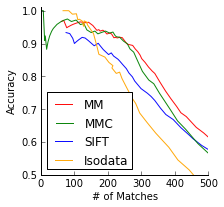
\includegraphics[width=1\columnwidth]{images/result_pitts}
	\end{subfigure}%
	\caption{Results for 100 patch pairs based on the image pair in 
	Figure~\ref{fig:pitts_source}.}
	\label{fig:result_pitts}
\end{figure}

In terms of computational complexity, \emph{Ratio}, \emph{MM}, and 
\emph{Isomatch} can be implemented in $O(n\log n)$, where $n$ is the 
total number of feature points. The performance of \emph{Spectral} is 
upper bounded by $O(n^{3/2})$. Our current \emph{MMC} implementation has 
a complexity of $O(n^2)$ due to the construction of a similarity matrix 
of the feature points.  However, it is possible to approximate this in 
$O(n\log n)$ using search trees.  

As for speed, Table~\ref{table:running_times} shows the running time of 
the four algorithms over 100 image pairs of $250\!\times\!250$ pixels.  
These numbers should be taken with a grain of salt, given that much of 
the code behind \emph{MMC} and \emph{Isomatch} is implemented in Python, 
whereas \emph{MM} and \emph{Ratio} make use of OpenCV to execute 
computationally intensive operations in C++, which makes them much 
faster. 

\begin{table}[htb]
\caption{Running times as tested on a Intel\textregistered\ Core\texttrademark\ i5-3550 CPU @ 
3.30~GHz with 8~GB memory.}
\label{table:running_times}
	\centering
%	\small
\begin{tabular}{r*{5}{c}}
\hline
	Algorithm: & \emph{Ratio} & \emph{MM} & \emph{MMC} %
& \emph{Isomatch} & \emph{Spectral}	\\
	\noalign{\smallskip} 
	%
	Running time (seconds): & 21 & 23 & 2722 & 1146 & 994\\
	\hline
\end{tabular}
\end{table}
